\documentclass[border=10pt]{standalone}
\usepackage[svgnames]{xcolor}
\usepackage{amsmath}
\usepackage{pgfplots}
\pgfplotsset{compat=newest}
\usepackage[sfdefault]{FiraSans}
\usepackage{FiraMono}
\renewcommand*\familydefault{\sfdefault}
\begin{document}
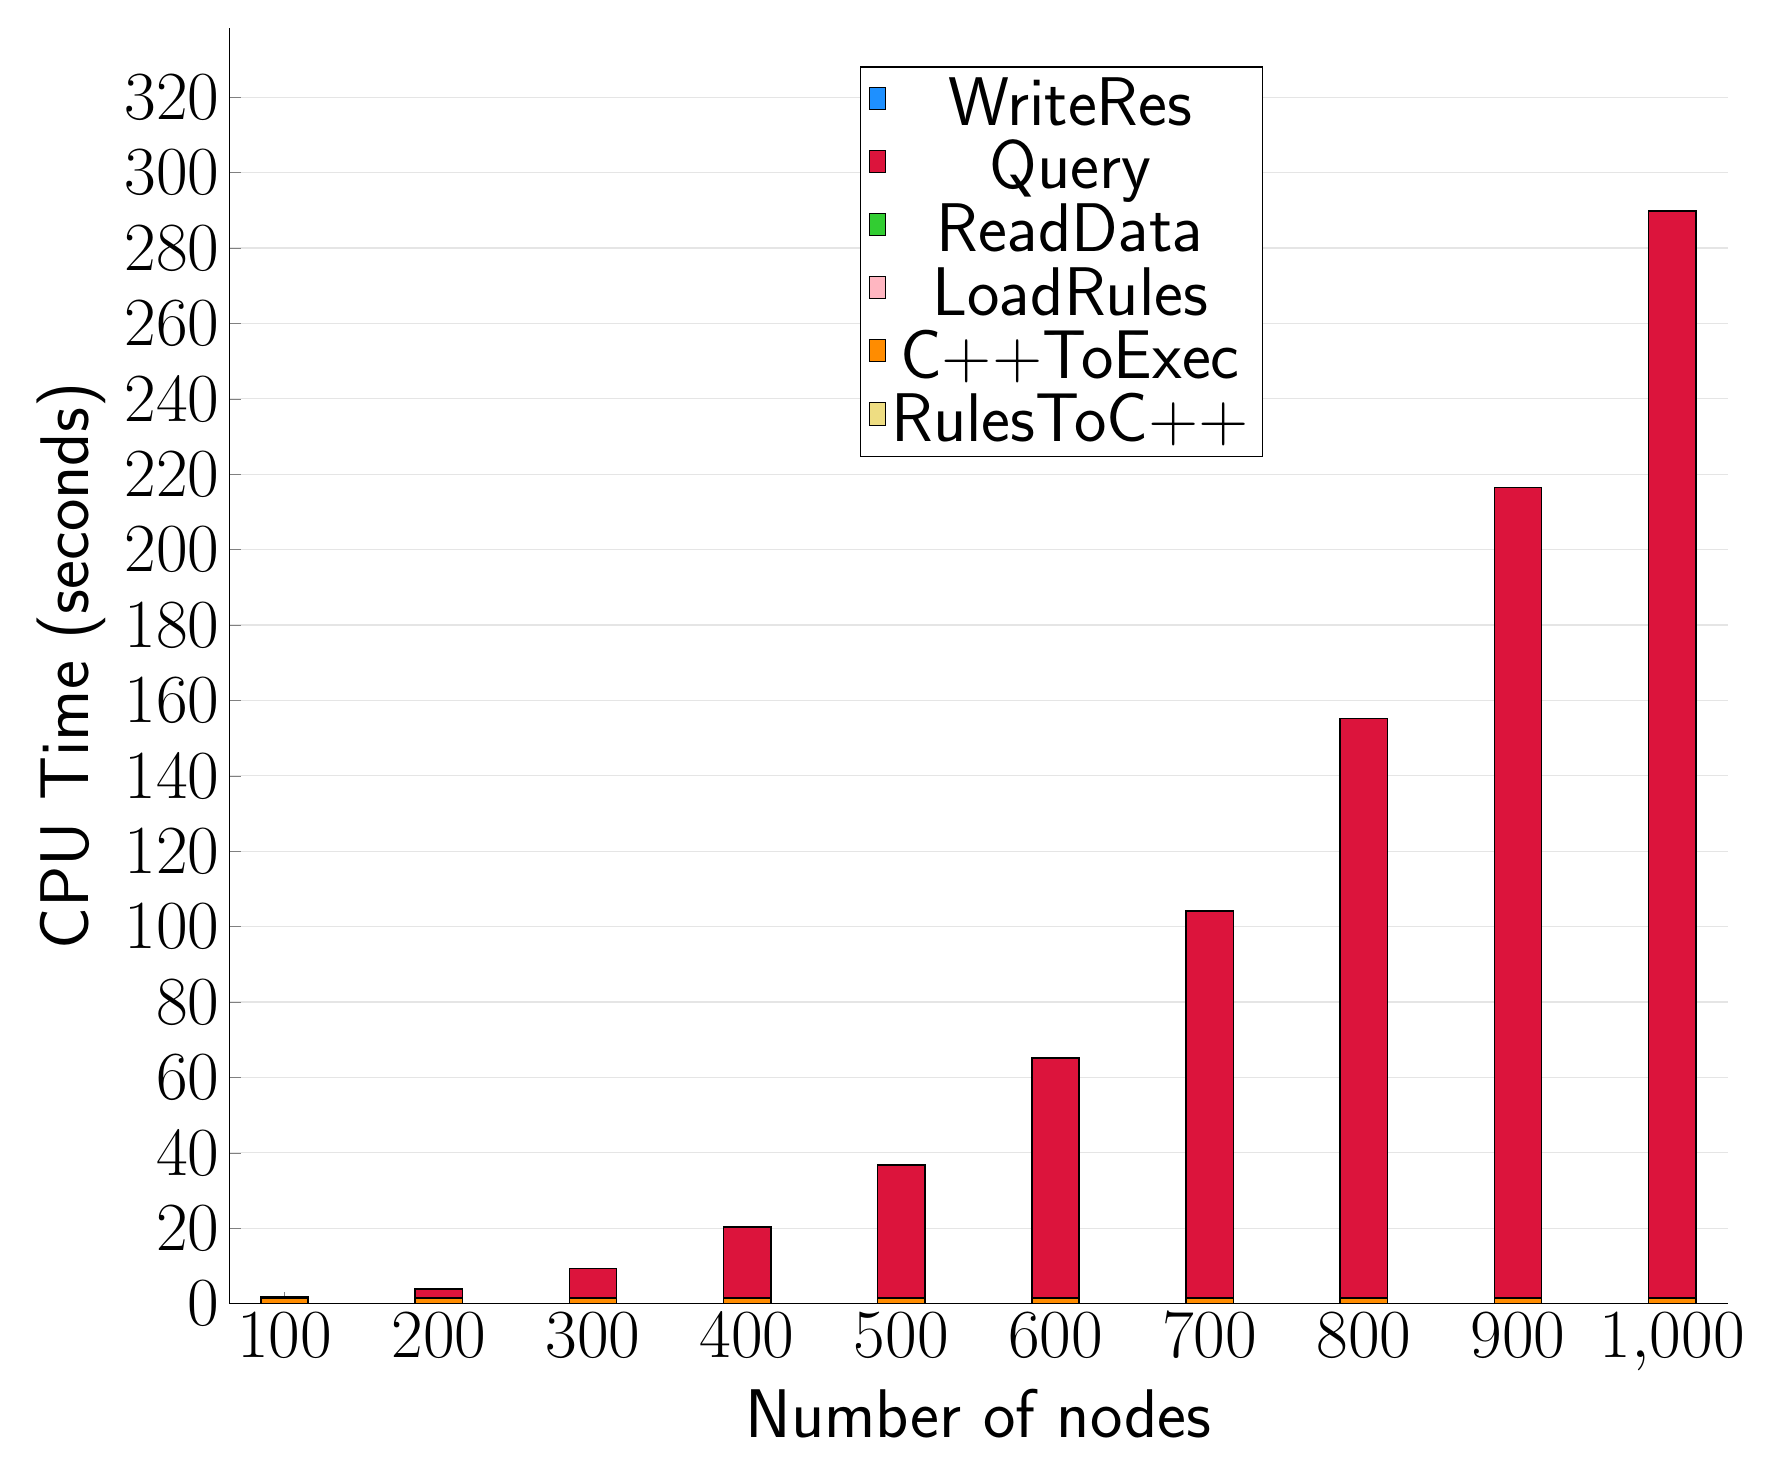
\begin{tikzpicture}
\begin{axis}[
   ybar stacked,
   width=1.7\textwidth,
   bar width=0.6cm,
   ymajorgrids, tick align=inside,
   major grid style={draw=gray!20},
   xtick=data,
   ymin=0, ymax=338.29920000000004,
   axis x line*=bottom,
   axis y line*=left,
   enlarge x limits=0.04,
   legend style={
       at={(0.69, 0.97)},
       anchor=north east,
       legend columns=1,
       font=\Huge,
   },
   ylabel={CPU Time (seconds)},
   xlabel={Number of nodes},
   label style={font=\Huge},
   tick label style={font=\Huge},
]
\addlegendimage{fill=DodgerBlue, draw=black, line width=0.2pt}
\addlegendentry{WriteRes}
\addlegendimage{fill=Crimson, draw=black, line width=0.2pt}
\addlegendentry{Query}
\addlegendimage{fill=LimeGreen, draw=black, line width=0.2pt}
\addlegendentry{ReadData}
\addlegendimage{fill=LightPink, draw=black, line width=0.2pt}
\addlegendentry{LoadRules}
\addlegendimage{fill=DarkOrange, draw=black, line width=0.2pt}
\addlegendentry{C++ToExec}
\addlegendimage{fill=LightGoldenrod, draw=black, line width=0.2pt}
\addlegendentry{RulesToC++}
\addplot +[fill=LightGoldenrod, draw=black, line width=0.55pt] coordinates {
(100, 0.008000000000000002)
(200, 0.006000000000000001)
(300, 0.010000000000000002)
(400, 0.006000000000000001)
(500, 0.004000000000000001)
(600, 0.0020000000000000005)
(700, 0.004000000000000001)
(800, 0.0020000000000000005)
(900, 0.0)
(1000, 0.0)
};
\addplot +[fill=DarkOrange, draw=black, line width=0.55pt] coordinates {
(100, 1.52)
(200, 1.53)
(300, 1.5220000000000002)
(400, 1.52)
(500, 1.528)
(600, 1.518)
(700, 1.518)
(800, 1.518)
(900, 1.52)
(1000, 1.5220000000000002)
};
\addplot +[fill=LightPink, draw=black, line width=0.55pt] coordinates {
(100, 0.00017759999999999998)
(200, 0.00016360000000000002)
(300, 0.0001526)
(400, 0.000158)
(500, 0.00015600000000000002)
(600, 0.0001626)
(700, 0.00016460000000000002)
(800, 0.0001732)
(900, 0.0001654)
(1000, 0.00016839999999999997)
};
\addplot +[fill=LimeGreen, draw=black, line width=0.55pt] coordinates {
(100, 0.0008738000000000001)
(200, 0.0012214)
(300, 0.0016288000000000001)
(400, 0.0020603999999999996)
(500, 0.0022374)
(600, 0.0028224)
(700, 0.0032372000000000004)
(800, 0.0035872)
(900, 0.0039324)
(1000, 0.0043104)
};
\addplot +[fill=Crimson, draw=black, line width=0.55pt] coordinates {
(100, 0.303342)
(200, 2.299058)
(300, 7.772150000000001)
(400, 18.77584)
(500, 35.29434)
(600, 63.59358000000001)
(700, 102.60619999999999)
(800, 153.7144)
(900, 214.94700000000003)
(1000, 288.29920000000004)
};
\addplot +[fill=DodgerBlue, draw=black, line width=0.55pt] coordinates {
(100, 0.00027020000000000006)
(200, 0.0003764)
(300, 0.00043119999999999996)
(400, 0.00037099999999999996)
(500, 0.0004332)
(600, 0.00038800000000000005)
(700, 0.0004084)
(800, 0.0004398)
(900, 0.0004963999999999999)
(1000, 0.00042259999999999997)
};
\end{axis}
\end{tikzpicture}

\end{document}
